\chapter{Foundations}
\label{chp:foundations}

This chapter provides information on overarching as well as foundational concepts relevant to the following chapters. Specifically, we cover two areas.

\begin{enumerate}
    \item \textbf{Scholarly Data}\\
        First, we give an overview of the academic publication ecosystem and its relation to the landscape of scholarly data. Understanding the parts involved and relations between them is helpful for understanding decisions made in the system design and method development of the approaches presented later on.
    \item \textbf{Data Mining \& Information Extraction}\\
        Second, we present relevant evaluation metrics from the areas of data mining and information extraction. These are essential for understanding the research goals as well as the results that were achieved.
\end{enumerate}

Explanations of concepts that are specific to the work presented in individual chapters, as well as an overview of state of the art approaches in the respective areas, are provided jointly with the approaches in Chapters \ref{chp:corpus}\,--\,\ref{chp:params}.

\section{Scholarly Data}

% What do I want to say and convey here?
% - what's the general nature of scholarly data?
%   -> structured representation of publication [meta]data that is the basis for (1) digital services in academia, (2) analyses, (3) ML model dev+evaluation
% - how is scholarly data generated
%   -> to some degree manually (metadata provided by authors), everything else (structured representations of full-text, references, etc.) out of necessity automated
% - what are the data sources and their peculiarities?
%   -> (see fig 2.1; from 3 stages of publishing, overall visual first, some special treatment for some metadata (wrt. access and requiring authors to manually provide it)
% - LaTeX; what is it, why is it not the end-all-be-all, and what endeavours have been there so far and are on the horizon of LaTeX development wrt. more structure and semantic information?
%   -> brief history, used primarily in STEM fields, Turing complete, document classes and packages provide semantic macros that translate in to visual representation but authors can always chose to directly describe visual presentation rather than semantic meaning, some endeavours to allow for more semantics (scholarly data specific and from accessibility POV)
% - What about other formats?
%   -> JATS is mighty, Word is XML, triple formats are used for metadata

\begin{figure}[bt]
  \centering
  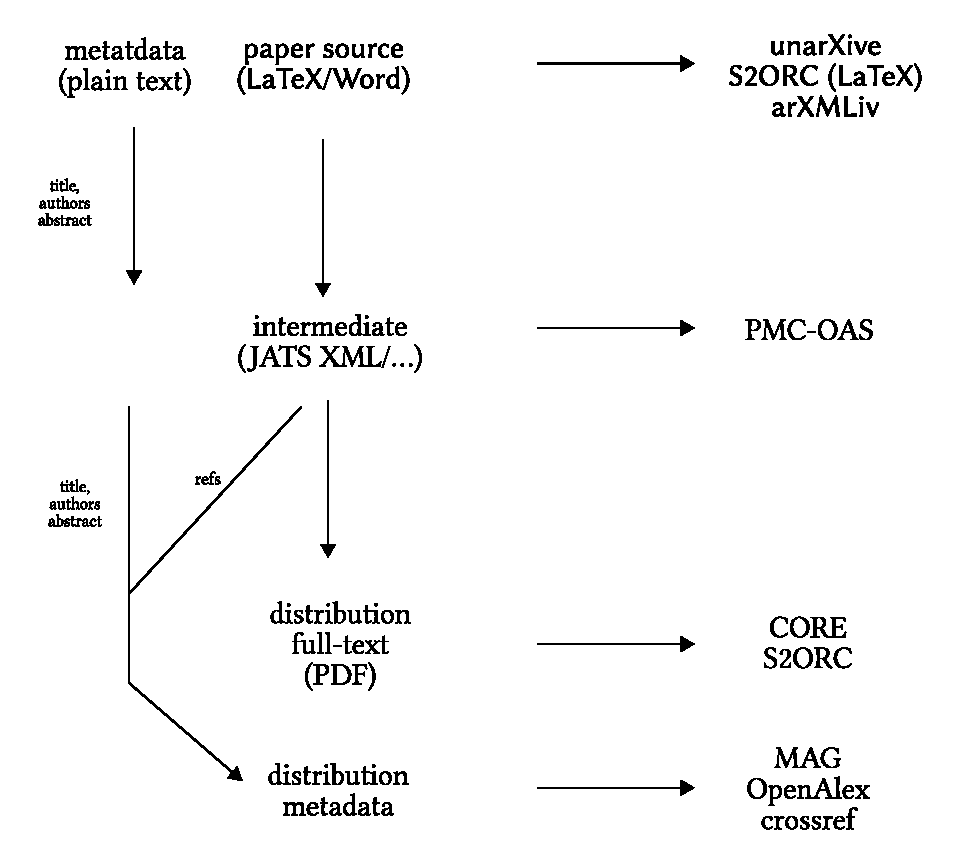
\includegraphics[width=0.7\linewidth]{figures/foundations/scholarly_data_lifecycle_dummy}
  \caption[Scholarly data lifecycle]{Scholarly data lifecycle (note: in text mention that for older publications it goes from some source to distribution on paper, and scholarly data then requires OCR on scanned documents)}
  \label{fig:foundations-datalifecycle}
\end{figure}

in Figure~\ref{fig:foundations-datalifecycle}

Joanne Cohn sending around e-prints~\cite{Feder2021,Turner2012}

June 1991 meets Paul Ginsparg who then goes on to start arXiv~\cite{Ginsparg2011a,Ginsparg2011}

arXiv used 1998 for scholarly IE~\cite{Nanba1998}

metadata dump since 2020(?) available on Kaggle~\cite{arxiv_kaggle_dataset}

\subsection{\LaTeX}

\subsection{Further Data Formats}

\paragraph{Word}

\paragraph{JATS XML}

\paragraph{PDF}

\paragraph{Triple Formats}
RDF, Turtle, JSON-LD, ... (relevant for metadata)

% document classes and packages provide semantic macros and translate them
% into visual output, but user can at any time also use visual primitives
% directly


\section{Data Mining \& Information Extraction}

% What do I want to say and convey here?
% - 

\subsection{Data Quality Metrics}

\subsection{Model Evaluation Metrics}
